\subsection{Task 3: Pressure Loss Before and After the Expansion}
\label{sec:task3intro}

In this part, the pressure loss after sudden and gradual expansions will be examined for our geometry. 
While doing so, different expansion ratios will be considered and simulated. In these calculations, equations, materials and tables from Frank M. White's fluid mechanics textbook \cite{white_chul_2016} will be used frequently.\\


\noindent The minor loss measured by the head loss is defined \cite{white_chul_2016} as:

\begin{equation}
    h_m = \frac{\Delta p}{\rho g}
    \label{eq:hm}
\end{equation}

\noindent where $\rho$ is the density of the fluid, $g$ is the gravitational acceleration and $\Delta p$ is $p_1 - p_2$ with those being the pressure values before and after the expansion of the pipe. Also to be used in our calculations, minor head loss coefficient is calculated as follows:

\begin{equation}
    K = \frac{h_m}{V^2 / (2g)}
    \label{eq:headlosscoeff}
\end{equation}

\noindent where K is the average velocity inside the pipe, that is, the velocity we have defined when creating the inlet boundary conditions and initial conditions. \\

\noindent For the sudden expansion case where the expanding walls are perpendicular to the centerline of the pipe, 3 simulations are done for different expansion ratios, that is, the ratio of smaller pipes radius and that of the bigger pipe's. The ratios which will be examined are as follows:

\begin{itemize}
    \item 0.2
    \item 0.4
    \item 0.6
\end{itemize}

\noindent In addition to this, instead of a sudden expansion a gradual expansion with expansion ratio of 0.4 and a expansion degree (the angle between the centerline of the pipe and the expansion walls) of $2\theta = 20^{\circ}$.


\begin{figure}[H]
  \centering
  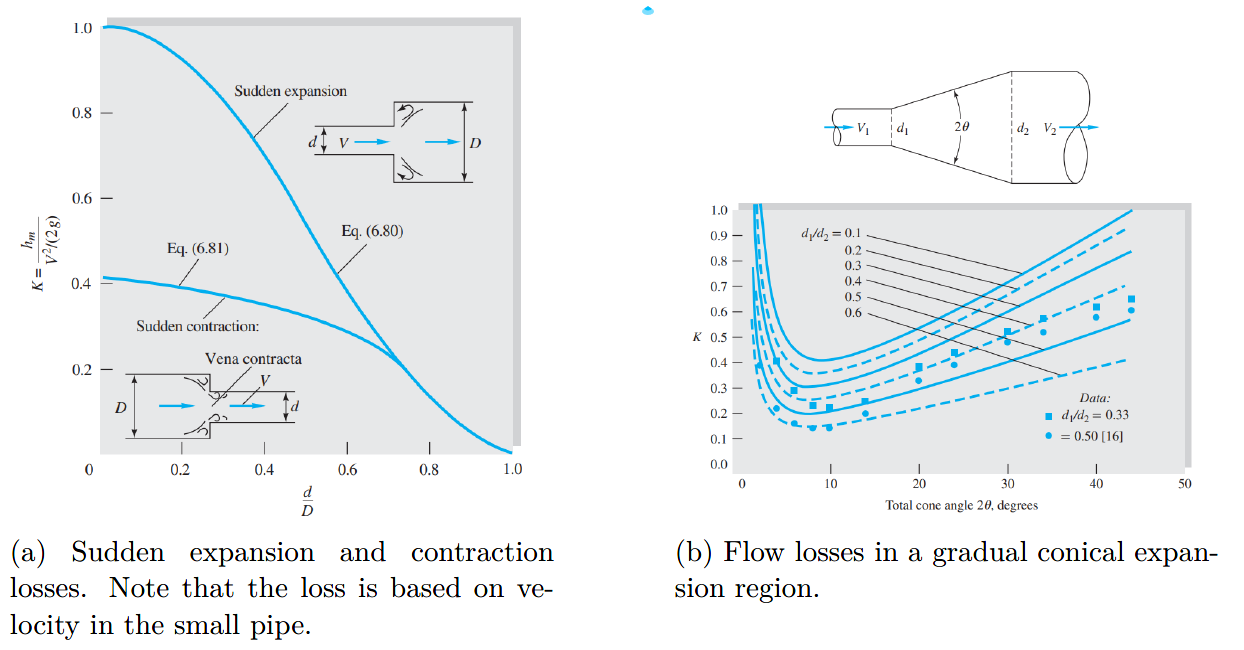
\includegraphics[width=.9\linewidth]{images/task3/expansion_figures.png}
  \caption{Expansion Plots \cite{white_chul_2016}}
  \label{fig:exp_plots}
\end{figure}


\noindent To validate and compare our results, plots that models these parameters from White's book \cite{white_chul_2016} will be used. Those plots can be seen from Figure \ref{fig:exp_plots}.